\documentclass{article}
%\usepackage{blindtext}
\usepackage{titlesec}
\usepackage{graphicx} % Required for inserting images
\usepackage{url} % formato de URLs
\usepackage{amsmath} 
\usepackage[colorlinks=true, linkcolor=blue, citecolor=blue, urlcolor=blue]{hyperref}
% Configuración de encabezados y pies de página
\usepackage{fancyhdr} % paquete para personalizar encabezados y pies de página
\usepackage[margin=2.5cm]{geometry}
\pagestyle{fancy}

\title{Simulación de Procesos de Conformado con Herramientas Open Source}
\author{Luciano Buglioni}
\date{December 2024}
\renewcommand*\contentsname{Contenidos}
\begin{document}

\maketitle
\tableofcontents
\newpage
\section{Introducción}
El presente documento tiene como objetivos introducir a los principales métodos de resolución computacional actuales para problemas de conformado en general, haciendo foco especialmente en los procesos de estampado y forja.

%\blindtext

\addcontentsline{toc}{section}{Unnumbered Section}

%blindtext

\section{Métodos}

Una razón del éxito del método de elementos finitos en el análisis multifísico es que es un método muy general. Resolver los sistemas de ecuaciones resultantes es igual o muy similar a los métodos bien conocidos y eficientes utilizados en el análisis estructural y electromagnético. Otra razón de su éxito es que facilita “aumentar el orden de los elementos,” lo que permite aproximar los campos físicos con gran precisión. Esto típicamente corresponde a aproximar localmente los campos físicos con polinomios de “orden superior,” como polinomios de segundo y tercer grado, o incluso mayores. Esta técnica es a menudo crítica, por ejemplo, en el caso de análisis de tensiones con alta precisión.
Si consideramos el ejemplo del análisis de tensiones, es bastante común que existan concentraciones importantes de tensión cerca de algunas esquinas de una pieza mecánica. En este caso, el método de elementos finitos permite dos formas diferentes de aumentar la precisión de la solución alrededor de esa esquina. Una forma es aumentar el orden de los elementos, como se describió anteriormente. Otra metodología consiste en refinar localmente la malla cerca de esa esquina; es decir, la densidad de los elementos aumenta localmente. Cuanto más fina sea la malla (es decir, más elementos), más precisa será la aproximación del campo de tensiones alrededor de la esquina de interés. Ambas técnicas se utilizan en los programas de elementos finitos y, con frecuencia, se automatizan desde la perspectiva del usuario. Esto se conoce como “refinamiento adaptativo de la malla.”
\subsection{Métodos de Malla}
\subsubsection{Elementos Finitos: FEM}

\subsubsection{Volúmenes Finitos: FVM}
\begin{equation}
\int_\Omega \frac{\partial (\rho \boldsymbol{v})}{\partial t} \; \text{d}\Omega = \oint_\Gamma \boldsymbol{n} \cdot \boldsymbol{\sigma} \; \text{d}\Gamma + \int_\Omega \rho \boldsymbol{b} \; \text{d}\Omega
\end{equation}

\subsection{Métodos sin Malla}

\subsubsection{SPH}

\subsection{Solvers Implícitos vs. Explícitos}

Las formulaciones de geometría lineales y no lineales pueden resolverse de manera explícita o implícita. En los enfoques explícitos, el término se calcula utilizando el campo de desplazamiento conocido en el paso de tiempo anterior. Como consecuencia, los enfoques explícitos no requieren la formación ni la solución de un sistema lineal, pero su tamaño de paso de tiempo está limitado por la condición de Courant–Friedrichs–Lewy(CFL). En cambio, los enfoques implícitos calculan el término utilizando el desplazamiento desconocido o una combinación del campo de desplazamiento desconocido y el campo de desplazamiento conocido del tiempo anterior. Como resultado, los métodos implícitos son incondicionalmente estables, sin restricciones en el tamaño del paso de tiempo, aparte del control de la precisión temporal.

Las ventajas relativas de los enfoques explícitos e implícitos se pueden resumir de la siguiente manera:

Ventajas del método explícito:
\begin{itemize}
\item Cada paso de tiempo es rápido, ya que no se resuelve un sistema lineal.
\item No hay problemas de convergencia, ya que no se requiere iteración en cada paso de tiempo; por lo tanto, los métodos explícitos tienden a ser robustos para tratar problemas altamente no lineales.
\item Los métodos explícitos tienen una excelente escalabilidad paralela, ya que no se resuelve un sistema lineal.
\end{itemize}
Desventajas:
\begin{itemize}
\item Para la mayoría de los materiales de ingeniería, la restricción del tamaño del paso de tiempo puede ser prohibitiva. En consecuencia, los métodos explícitos suelen ser eficientes solo para problemas rápidos, que ocurren en períodos de tiempo cortos.
\end{itemize}

Ventajas del método implícito:
\begin{itemize}
\item 
La capacidad de usar pasos de tiempo grandes significa que los problemas lentos (es decir, estáticos o cuasi-estáticos) pueden analizarse de manera eficiente.
\end{itemize}
Desventajas:
\begin{itemize}
\item 
Para problemas altamente no lineales (por ejemplo, contacto por fricción, grandes deformaciones, plasticidad, fractura), los métodos implícitos pueden tener dificultades para converger.
\end{itemize}


\subsection{Solvers Acoplados vs. segregados}
Generalmente para resolver la ecuación de cantidad de movimiento debe resolverse lo siguiente:\\
\begin{equation}
\frac{\partial (\rho \boldsymbol{v})}{\partial t} = \boldsymbol{\nabla} \cdot \boldsymbol{\sigma} + \rho \boldsymbol{b}
\end{equation}

Segregado: Suele ser el método más común en los solvers explícitos, y en aproximaciones como Solids4FOAM

En el método segregado, el término se aproxima implícitamente como un término de Laplaciano, donde las correcciones diferidas explícitas aseguran que la ecuación gobernante original se cumpla en la convergencia. La ventaja de este enfoque es que desacopla temporalmente las direcciones x, y y z de la ecuación de momento, lo que resulta en un enfoque eficiente en términos de memoria. Una desventaja de este enfoque es que la convergencia de las iteraciones externas puede ser lenta en casos cuasi-estáticos, donde la geometría tiene una alta relación de aspecto, por ejemplo, en una viga en voladizo doblándose.

Acoplado: El enfoque acoplado o acoplado por bloques tiene como objetivo maximizar el tamaño del término implícito al incluir implícitamente el acoplamiento entre componentes dentro de la ecuación de momento. La ventaja del enfoque acoplado es que la convergencia suele ser más rápida que el enfoque segregado en problemas cuasi-estáticos y estáticos; sin embargo, para problemas transitorios, el enfoque segregado puede ser más competitivo, ya que la superior convergencia del enfoque acoplado puede verse compensada por el tiempo adicional necesario para formar y resolver el sistema acoplado. En el caso especial de geometría lineal, elasticidad lineal y condiciones de frontera lineales, el enfoque acoplado converge en una iteración externa, ya que el problema es lineal.

Semi-Acoplado: Los enfoques semi-acoplados se encuentran entre los enfoques segregados y acoplados. Uno de estos enfoques introduce la presión hidrostática como una incógnita adicional, donde el desplazamiento (o velocidad) y la presión se tratan implícitamente de manera acoplada, mientras que el acoplamiento entre componentes del desplazamiento en la ecuación de momento aún se trata explícitamente de manera diferida. Estos enfoques semi-acoplados son similares a los enfoques acoplados utilizados en los solucionadores de fluidos, por ejemplo, pUCoupledFoam en foam-extend.


\section{Herramientas Actuales}
\subsection{Interfaz Gráfica}
Se está desarrollando una interfaz gráfica desde cero, que sirve para armar los inputs de los modelos y exportarlos a los diferentes solvers. Este programa tiene la facilidad de poder insertar scripts de python para automatizar las acciones, lo cual lo hace muy robusto. En este \href{https://github.com/luchete80/WeldFormGUI}{enlace} se presenta el repositorio, y se muestra a continuación una imagen de la interfaz.
\\
\begin{figure}
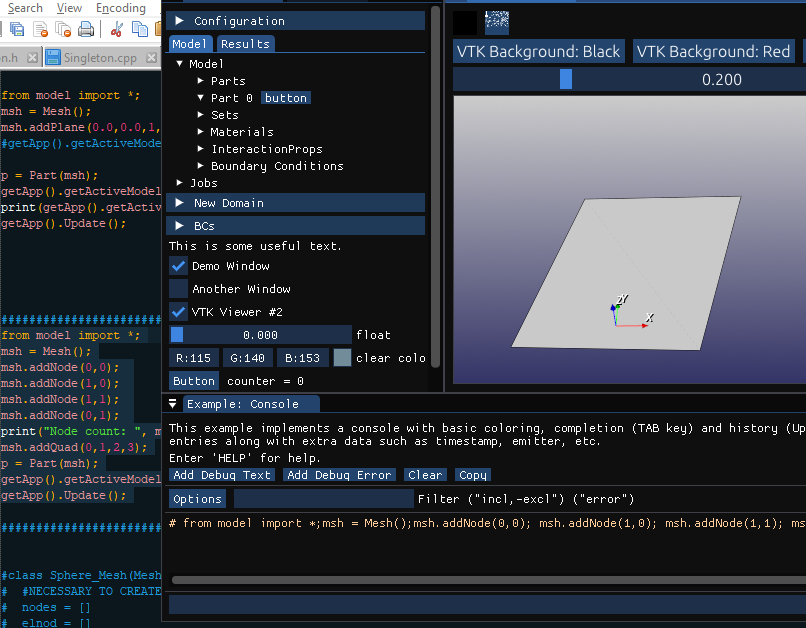
\includegraphics[width=0.9\textwidth]{images/20241114.png}
\end{figure}

A continuación se muestra un resumen de las diferentes herramientas utilizadas según el proceso. 

\begin{figure}
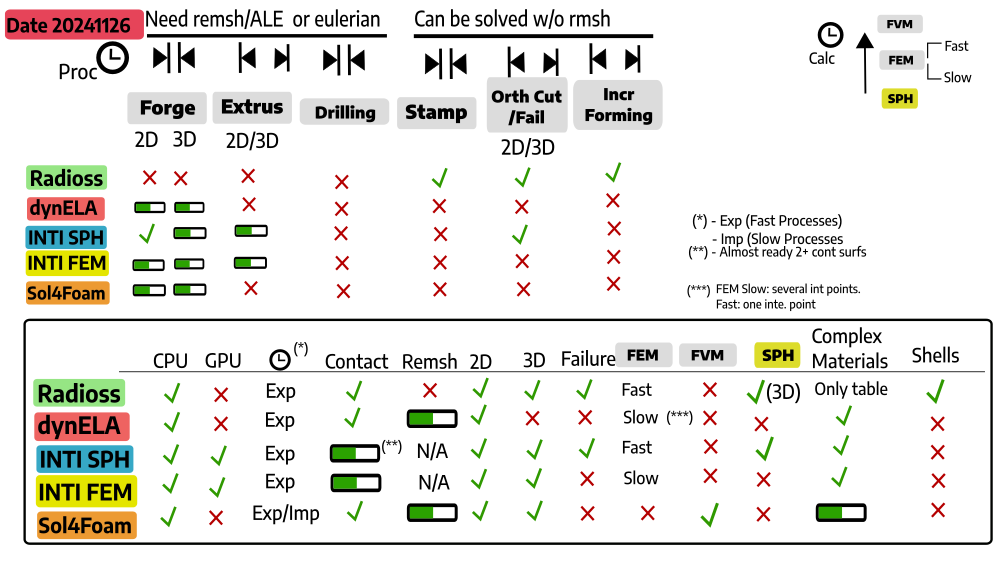
\includegraphics[width=1.0\textwidth]{images/20241126_Tools.png}
\end{figure}

\subsection{Solvers FEM}

\subsubsection{OpenRadioss - Terceros}
OpenRadioss es un software FEM (aunque también tiene módulos de FVM y SPH), cuyo fuerte es el módulo explícito. Es un referente en las simulaciones de impacto de vehículos, y es el competidor directo de ANSYS LS-Dyna. Suele utilizar elementos de integración reducida. 

\subsubsection{ReDynELA - Terceros, fuertemente adaptado}
Este solver trabaja con elementos de tipo lineal, es explícito y es escrito por Olivier Pantalé. 

\subsection{Volúmenes Finitos (FVM)}
\subsubsection{Solids4Foam}


\subsection{Solvers SPH}
\subsubsection{WeldFormSPH-CPU}
Esta herramienta fue desarrollada prácticamente desde cero por los autores, a partir de la herramienta \href{https://github.com/mghkorzani/persiansph}{PersianSPH}. Se han escrito alrededor de 40 mil lineas de código desde el proyecto original. Calcula por el método SPH procesos que involucran contacto, acoplamiento térmico, y materiales de \textit{Johnson Cook, Hollomon}. Se han obtenido resultados muy aceptables para proceso de extrusión axilsimétrico, que se muestran en la figurea.
\begin{figure}
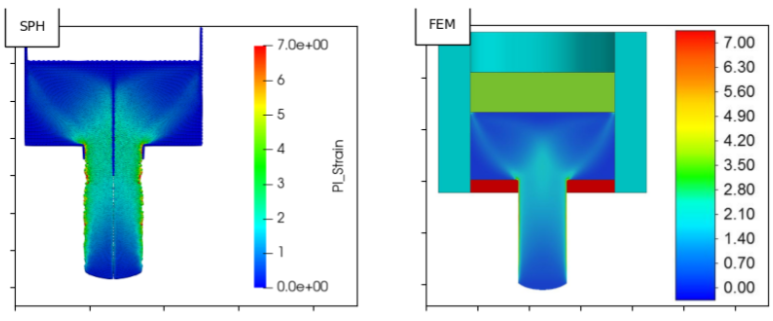
\includegraphics[width=0.7\textwidth]{images/20240723_01.png}
\end{figure}
En este \href{https://github.com/luchete80/weldform}{link} se encuentra el código fuente listo para compilar. 

\subsubsection{WeldFormSPH-GPU - Propio}
Este solver está paralelizado para correr en la placa gráfica, y está escrito en CUDA C++.
En este link puede bajarse el código para compilar.
\href{https://github.com/luchete80/weldformGPU}{WeldFormGPU}
\section{Referencias}
https://www.machinedesign.com/additive-3d-printing/fea-and-simulation/article/21832072/whats-the-difference-between-fem-fdm-and-fvm 

https://www.solids4foam.com/documentation/solid-models.html

\section{Bibliografía Recomendada}
Método FEM:
\begin{itemize}
\item
Finite Element Procedures - Jlaus Jurgen. Bathe
\end{itemize}
\par

Método FVM:
\begin{itemize}
\item
Computational Methods for Fluid Dynamics. Ferzinger \& Peric.
\end{itemize}



\end{document}
